
\documentclass[./00_PhotoBox.tex]{subfiles}
\graphicspath{{\subfix{./img/}}}
\begin{document}


\chapter{Photogrammmetrischer Hintergrund}
\label{c:photogrammmetrie}
Das Erzeugen des 3D-Modelles basiert auf der Verknüpfung von Bildern aus verschiedenen Positionen über identische Punkte. Hieraus können dann die Orientierung der Kameras zueinander und die Koordinaten der Punkte in einem lokalen Koordinatensystem ohne bekannten Maßstab berechnet werden. Durch die Nutzung von bekannten Größen beispielsweise durch Maßstäbe kann dieses System transformiert werden.

Dieses Kapitel beschreibt die hierfür notwendigen Bedingungen und die Grundlagen der Rekonstruktion des Objektes als 3D-Modell.

\begin{figure}
    \centering
    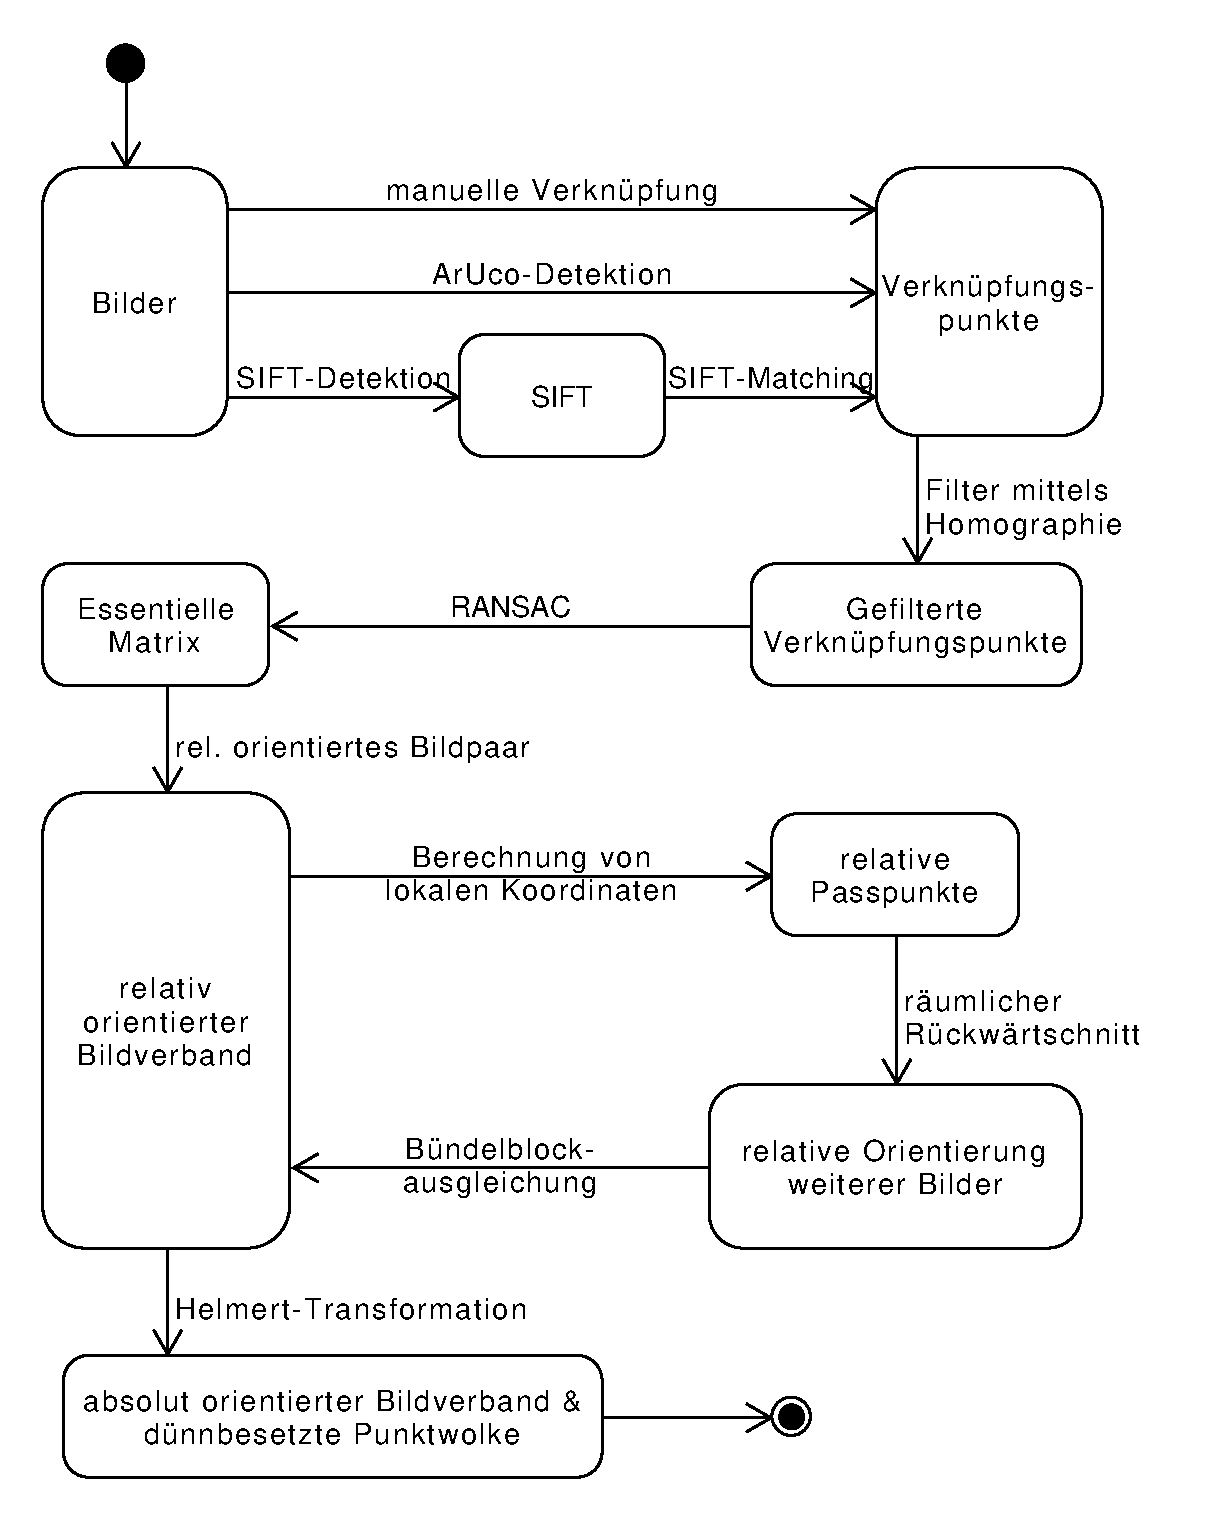
\includegraphics[width=0.8\textwidth]{./img/Ablauf.pdf}
    \centering
    \caption{Ablauf der Bildverknüpfung, nach \citealt[S. 492]{luhmann}} %Bildunterschrift
    \label{img:ablauf} %ID fürs Bild
\end{figure}

\section{Innere Orientierung}
\label{s:innereorientierung}
Aus der Position eines Punktes in einem Bild kann vereinfacht gedacht ähnlich einer Messung mit einem Theodolit die Richtung des Punktes in Relation zu der Kamera bestimmt werden. Damit diese Berechnung möglich wird, müssen die Parameter der Kamera bekannt sein, die sogenannte innere Orientierung. Sie beschreibt die Abbildung der Kamera mathematisch. Wichtigste Parameter sind hierbei die Lage des Bildhauptpunktes und die Kamerakonstante. Außerdem zählen hierzu auch die Parameter, die die Bildfehler wie die Verzeichnung, beschreiben. \citep[S. 179f]{luhmann}

Die innere Orientierung kann während der Messung beispielsweise mittels Bündel\-block\-ausgleichung bestimmt werden. Bedingung hierfür ist jedoch, dass die innere Orientierung stabil ist und sich nicht während der Messung ändert \citep[S. 181f]{luhmann}.

Jede Einstellung der Kameraoptik verändert die innere Orientierung und auch jede Kamera,auch einer Modellreihe, kann je nach Genauigkeitsanspruch als unterschiedlich angesehen werden. Änderungen können sich beispielsweise durch Umfokussierung oder die Nutzung eines optischen Zoom ergeben, aber auch durch einen mechanisch instabilen Aufbau der Kameras. Daher sollten die Bilder möglichst mit einer Kamera mit festen Einstellungen (Brennweite, Fokus, Blende, Objektiv) aufgenommen werden. Änderungen der Empfindlichkeit (ISO-Zahl) oder Belichtungszeit sind unproblematisch für die innere Orientierung \citep[S. 176]{luhmann}.


\section{Bilder}
\label{s:bilder}

Die Berechnung der Tiefeninformationen ist nur möglich, sofern der Punkt in mindestens einem weiteren Bild abgebildet ist. Die Genauigkeit der Berechnung ist vom Schnittwinkel dieser beiden Strahlen abhängig. Um möglichst gute Schnitte zur Ver\-fügung zu haben und die innere und äußere Orientierung möglichst gut berechnen zu können, müssen diese Bilder einige Bedingungen erfüllen.

\subsubsection{Überlappung und Bildinhalte}
Da die Bilder durch identische Punkte verbunden werden, müssen die Bildinhalte sich überlappen. Die automatische Identifikation von identischen Punkten ist auf verschiedene Weisen möglich: Entweder durch die Nutzung von codierten Passpunkten wie ArUco-Markern oder konzentrischen Passpunkten nach \cite{schneider}. Alternativ können auch eine Merkmalsextraktion zur Indentifikation von gemeinsamen Punkten genutzt werden, beispielsweise durch die SIFT-Methode. Hierfür muss die oberfläche aber genügend Texturen aufweisen. \citep[S. 478]{luhmann}

\subsubsection{Belichtung}
und bei sich stark ändernden Helligkeitsverhältnissen auch hilfreich, jedoch wird hierdurch auch die Helligkeit der Verknüpfungspunkte verändert, was wiederum problematisch sein kann. Entsprechend ist es empfehlenswert bei gleichmäßiger Beleuchtung, die sich auch nicht ändern sollte, die Bilder zu erstellen - also beispielsweise bei bedeckten Himmel.

\subsubsection{Position und Ausrichtung der Kamera}
Bilder, die vom gleichen Standpunkt aufgenommen wurden, sind oft nur ungenau verknüpfbar. Daher empfiehlt es sich, eher um Objekte herum zu gehen, statt beispielsweise bei Innenräumen sich nur in die Mitte zu stellen und sich zu drehen. Während der Aufnahmen sollte die Kamera natürlich möglichst ruhig gehalten werden, um möglichst scharfe Bilder zu generieren. Dies ist vor allem bei UAV-Flügen relevant, die auch aus hoher Geschwindigkeit Bilder aufnehmen könnten. Jedoch weisen die meisten Digitalkamera einen Rolling-Shutter-Effekt auf, dass heißt die Bildreihen werden nicht alle zeitgleich aufgenommen, sondern die oberen vor den unteren. Daher ist es sinnvoll, das UAV kurz schweben zu lassen und dann ein Bild zu machen. \citep[S. 147]{opendronemap}

Umso weiter die Kamera vom Objekt entfernt ist, umso mehr Inhalte und entsprechend mehr Verknüpfungsmöglichkeiten sind im Bild enthalten. Daher sollte sich immer klar gemacht werden, welche Auflösung benötigt wird und entsprechend die Entfernung bzw. bei UAV-Aufnahmen die Höhe zu wählen. Der Abstand sollte außerdem variiert werden, da dieses bei der Ausgleichung der inneren Orientierung hilft. \citep[S. 144f]{opendronemap}

\subsubsection{Schärfentiefe und Fokussierung}


\section{Verknüpfungspunkte}
Um die einzelnen Bilder verknüpfen zu können, werden identische Punkte zwischen zwei oder mehr Bildern benötigt. Diese können klassisch per Hand erfasst werden, jedoch ist dieses schon bei kleineren Projekten sehr zeitaufwändig. Daher wurde zusätzlich die Möglichkeit genutzt, automatisch Verknüpfungspunkte zu erzeugen.

\subsection{ArUco-Marker}
Eine Variante der automatischen Verknüpfungspunkte sind die sogenannten ArUco-Marker. Diese werden häufig für die Orientierung bei Augmented-Reality-Anwend\-ungen genutzt. OpenCV unterstützt die Erkennung dieser Marker. Sie werden als codierte Messmarken verwendet und können automatisch im Subpixelbereich erkannt werden. Jede Ecke kann hier einzeln identifiziert werden, sodass ein erkannter Marker vier Verknüpfungspunkte liefern kann.

\subsection{SIFT}
Die SIFT-Methode liefert Verknüpfungspunkte aus Mustern auf den photographierten Oberflächen. Es ist meist nicht notwendig explizit Marker an dem aufzunehmenden Objekt anzubringen, sofern seine Oberfläche nicht strukturlos ist (glatte weiße Wände etc.) oder in Bewegung ist.

Zur Erkennung von Merkmalen setzt das Verfahren auf die Detektion von Kanten. Diese werden in verschiedenen Stufen einer Bildpyramide erkannt und ihre Extrema berechnet. Es werden diese Merkmale weiter ausgedünnt, beispielsweise über den Kontrast. Sofern ein möglicher Marker identifiziert wurde, wird eine Beschreibung erzeugt. Diese erfolgt  durch Analyse der Helligkeitsabweichungen zu den Nachbar-Pixeln und wird an der stärksten Abweichung ausgerichtet. Hierdurch wird die Beschreibung dann richtungsunabhängig. Mit diesen kann dann die Übereinstimmung von zwei Markern in zwei Photos bestimmt werden, auch wenn die Bilder zueinander gekippt oder gedreht sind.
\citep[S. 483]{luhmann4}

\section{Verknüpfung von Bildern}
\label{s:photogramm}
Durch die drei beschriebenen Verfahren und die hieraus entstandenen Verknüpfungs\-punkte können die Bilder miteinander verknüpft werden. Da durch GNSS nur eine sehr grobe und ggf. auch falsche Vorausrichtung besteht, kann diese nur als sehr grobes Hilfsmittel genutzt werden. In diesen Ansatz wird es nur für die Beschränkung der SIFT-Detektion auf Bilder, die nahe beieinander sind oder sich ArUco- oder manuelle Punkte teilen, genutzt.
Für die eigentliche Verknüpfung werden dann nur photogrammmetrische Verfahren genutzt. Über diese wird im Folgenden ein kurzer Überblick gegeben.

\begin{comment}
\subsection{Homographie}
grobe Filterung
\end{comment}

\subsubsection{Abbildungsgleichung}
\label{ss:abbildungsgleichung}
Die Abbildung eines Punktes auf einem Bild wird durch die Abbildungsgleichung beschrieben. In der Matrizenrechnung ergibt sich dieser aus der Multiplikation mit der Projektionsmatrix $P$. Diese ergibt sich aus der Kameramatrix $K$, der Rotation $R$ und dem Projektionszentrum $X_0$. (siehe \autoref{abbildungsgleichung}, nach \citealp[S. 244]{hartley} und \citealp[S. 288]{luhmann4})

\begin{align}
    \label{abbildungsgleichung}
    x' & = P \cdot X       \\
    P  & = K \cdot [R|X_0] \\
    P  & =
    \begin{bmatrix}
        c_x & 0   & x'_0 \\
        0   & c_y & y'_0 \\
        0   & 0   & 1
    \end{bmatrix}
    \cdot
    \begin{bmatrix}
        r_11 & r_21 & r_31 & X_0 \\
        r_12 & r_22 & r_32 & Y_0 \\
        r_13 & r_23 & r_33 & Z_0 \\
    \end{bmatrix}
\end{align}

Um die Beziehung zwischen zwei Bildern aufzustellen, kann man die Abbildungsgleichung nutzen. Da es hier nur um die Beziehung zwischen zwei Bildern geht, kann die Rotation und Translation des ersten Bildes auf 0 gesetzt werden ($R$ ist dann eine 3x3-Einheitsmatrix und $X_0$ ein Nullvektor). $X_0$ des zweiten Bildes wird zur Translation zwischen den beiden Bildern. \citep[S. 326]{luhmann4}

\subsubsection{Fundamental-/Essentielle Matrix}
Die Fundamentalmatrix beschreibt das Verhältnis von identischen Punkten in zwei Bildern zueinander. Sie kann genutzt werden, um die Drehung und Verschiebung zwischen zwei Aufnahmeorten zu bestimmen. Die Formel für die Fundamentalmatrix lautet:
\begin{align}
    x'^T \cdot F \cdot x'' & = 0
\end{align}
Sie unterscheidet sich nur von der Essentiellen Matrix in der Eigenschaft, dass bei der Essentiellen Matrix die Kameraparameter bekannt sein müssen. Diese werden dann auf die Bildkoordinaten angewendet und $x'$ und $x''$ werden so unabhängig (normalisiert) von den Kameraeinstellungen. Mittels Singulärwertzerlegung lässt sich dann die Rotation und Translation aus der Essentiellen Matrix bestimmen. Im Falle von Bildern die mit Digitalkameras aufgenommen wurden sind die Kameraparameter zumindest näherungsweise aus den EXIF-Daten der Bilder bekannt, sodass dieser Weg hier genutzt werden kann. \citep[S. 257]{hartley}

In der entstandenen Software wurde die Methode verwendet, um die Verknüpfung des Startpaares zu errechnen.

\subsection{Fundamental-/Essentielle Matrix}
Die Fundamentalmatrix beschreibt das Verhältnis von identischen Punkten in zwei Bildern zueinander. Sie kann genutzt werden, um die Drehung und Verschiebung zwischen zwei Aufnahmeorten zu bestimmen. Die Formel für die Fundamentalmatrix lautet:
\begin{align}
    x'^T \cdot F \cdot x'' & = 0
\end{align}
Sie unterscheidet sich nur von der Essentiellen Matrix in der Eigenschaft, dass bei der Essentiellen Matrix die Kameraparameter bekannt sein müssen. Diese werden dann auf die Bildkoordinaten angewendet und $x'$ und $x''$ werden so unabhängig (normalisiert) von den Kameraeinstellungen. Mittels Singulärwertzerlegung lässt sich dann die Rotation und Translation aus der Essentiellen Matrix bestimmen. Im Falle von Bildern die mit Digitalkameras aufgenommen wurden sind die Kameraparameter zumindest näherungsweise aus den EXIF-Daten der Bilder bekannt, sodass dieser Weg hier genutzt werden kann. \citep[S. 257]{hartley}

In der entstandenen Software wurde die Methode verwendet, um die Verknüpfung des Startpaares zu errechnen.

\subsection{Vorwärtsschnitt}
Aus den zwei Projektionsmatrizen zweier Bilder und der Position eines identischen Punktes in beiden Bildern lassen sich dann lokale (Modell-)Koordinaten des Punktes berechnen. Da auch dieses nicht fehlerfrei ist, wurde hierfür die Methode der linearen Triangulation verwendet. Hierbei wird der entstehende Fehler ausgeglichen. \citep[S.312]{hartley}

\subsection{Rückwärtsschnitt}
Entsprechend lässt sich auch aus der Position von Punkten mit bekannten lokalen Koordinaten die Position und Drehung eines Bildes berechnen. Dieses wurde genutzt, um weitere Bilder an das Startpaar heranzuknüpfen. Hierfür werden mindestens 5 Punkte benötigt. \citep[S. 533ff]{hartley}


\section{Bündelblockausgleichung}
Mittels Bündelblockausgleichung können die grob mit den vorher genannten Verfahren bestimmten Positionen und Drehungen in einer Ausgleichung optimiert werden. Hierzu gehen alle Parameter der Bilder und die Positionen der Passpunkte in die gemeinsame Ausgleichung ein. Grundlage der Ausgleichung ist die in \autoref{ss:abbildungsgleichung} beschriebene Abbildungsgleichung. Als Ergebnis erhält man die ausgeglichenen Parameter und Genauigkeitsangaben für diese. \citep[S. 340]{luhmann4}


\end{document}